\documentclass[conference]{IEEEtran}
\IEEEoverridecommandlockouts

\usepackage{cite}
\usepackage{amsmath,amssymb}
\usepackage{graphicx}
\usepackage{booktabs}
\usepackage{array}
\usepackage{textcomp}
\usepackage{xcolor}
\usepackage[hyphens]{url}
\usepackage{tikz}
\usetikzlibrary{arrows.meta,positioning,calc,fit,backgrounds}
\usepackage{fontspec}
\setmainfont{texgyretermes-regular.otf}[BoldFont=texgyretermes-bold.otf,ItalicFont=texgyretermes-italic.otf,BoldItalicFont=texgyretermes-bolditalic.otf]
\setsansfont{texgyreheros-regular.otf}[BoldFont=texgyreheros-bold.otf,ItalicFont=texgyreheros-italic.otf,BoldItalicFont=texgyreheros-bolditalic.otf]
\setmonofont{texgyrecursor-regular.otf}[Scale=0.9]
\usepackage{unicode-math}
\setmathfont{texgyretermes-math.otf}
\usepackage{microtype}

\linespread{1.16}
\setlength{\textfloatsep}{14pt plus 2pt minus 4pt}
\setlength{\floatsep}{12pt plus 2pt minus 2pt}
\setlength{\intextsep}{12pt plus 2pt minus 2pt}
\setlength{\abovecaptionskip}{4pt}
\setlength{\parskip}{1.5pt}
\newcommand{\AUC}{0.977}
\newcommand{\AUClo}{0.973}
\newcommand{\AUChi}{0.981}
\newcommand{\EER}{6.2}
\newcommand{\EERlo}{5.5}
\newcommand{\EERhi}{7.0}
\newcommand{\EERthr}{0.0102}
\newcommand{\AccEER}{93.8}
\newcommand{\EERexcl}{3.2}
\newcommand{\AUCexcl}{0.996}
\newcommand{\EERseen}{0.3}
\newcommand{\EERunseen}{3.3}
\newcommand{\AUCunseen}{0.995}
\newcommand{\AUCAsev}{0.725}
\newcommand{\EERAsev}{34.4}
\newcommand{\EERAsevlo}{30.4}
\newcommand{\EERAsevhi}{38.4}
\newcommand{\DetAsev}{1.2}
\newcommand{\DetOther}{89.3}
\newcommand{\ECE}{0.083}
\newcommand{\Brier}{0.076}
\newcommand{\NLL}{0.425}
\newcommand{\FPRhalf}{0.8}
\newcommand{\FNRhalf}{16.8}
\newcommand{\TrainMinutes}{15.7}
\newcommand{\SecPerEpoch}{157}
  % macros generated from the saved run files by gen_tex.py

\graphicspath{{figures/}}
\def\BibTeX{{\rm B\kern-.05em{\sc i\kern-.025em b}\kern-.08em T\kern-.1667em\lower.7ex\hbox{E}\kern-.125em X}}

\begin{document}

\title{Face, Voice, or Both: An Audio-Visual Deepfake Detection Framework and a Voice-Branch Study on ASVspoof~2019}

\author{\IEEEauthorblockN{Author One\IEEEauthorrefmark{1}, Author Two\IEEEauthorrefmark{1}}
\IEEEauthorblockA{\IEEEauthorrefmark{1}Department of Computer Science and Engineering, University Name, City, Country\\
Email: author.one@university.edu, author.two@university.edu}}

\maketitle

\begin{abstract}
A manipulated video can carry a synthetic face, a cloned voice, or both, yet most detectors inspect a single channel and are tested on clean clips drawn from the same generators they were trained on. This paper describes a modular audio-visual detector built with both gaps in mind. It pairs an EfficientNet-B0 face branch with a ResNet-18 log-mel voice branch, offers rule-based and learned fusion, and ships a degradation protocol and Grad-CAM explanations. The pipeline is implemented, unit-tested and publicly released. We report the first completed experiment: the voice branch, trained on a class-balanced subset of ASVspoof~2019 LA (5{,}000 clips per partition) and scored once on the official evaluation partition, where eleven of thirteen attack systems never appear in training. The model reaches an AUC of \AUC{} (95\% CI \AUClo--\AUChi) and an equal error rate (EER) of \EER\% (\EERlo--\EERhi\%). Errors are concentrated rather than spread out: attack A17 is flagged in only \DetAsev\% of its clips at the default threshold, and removing it lowers the pooled EER to \EERexcl\%. Validation AUC reached 1.0 by the third epoch and therefore gave no warning of this gap. The visual, fusion and robustness experiments await dataset access and are specified here as a protocol.
\end{abstract}

\begin{IEEEkeywords}
deepfake detection, audio anti-spoofing, multimodal fusion, ASVspoof~2019, generalisation, calibration, Grad-CAM
\end{IEEEkeywords}

%--------------------------------------------------------------------
\section{Introduction}
\IEEEPARstart{G}{enerative} models can now swap a face, replay another person's expressions, or clone a voice from a few seconds of speech. Combined, they let an attacker impersonate someone in both channels at once. A detector that is useful outside a laboratory has to answer three practical questions. Which channel was altered? Does the answer survive the re-encoding that every sharing platform applies? And can a human reviewer see why the system decided as it did?

Existing work answers these questions unevenly. Face-forensics benchmarks \cite{rossler2019ff,li2020celebdf,dolhansky2020dfdc} and speech anti-spoofing challenges \cite{wang2020asvspoof} grew up separately, so face detectors ignore the soundtrack and speech countermeasures ignore the picture. Cross-dataset studies repeatedly show that a high score on the training distribution says little about performance on new generators \cite{yan2023deepfakebench,muller2022generalize}, and a recent in-the-wild benchmark reports AUC losses of roughly half for both video and audio detectors compared with earlier test sets \cite{chandra2025evaluation}. Decision thresholds and probability calibration, which determine what a deployed system actually flags, receive far less attention than ranking metrics.

This paper makes four contributions.
\begin{enumerate}
\item \textbf{Framework.} A modular pipeline, from dataset download to demo, with a face branch, a voice branch and two fusion schemes. The code base has an automated test suite and fixed random seeds.
\item \textbf{Label-aware fusion.} A formulation in which the overall label is ``fake if either channel is fake'', which motivates max and noisy-OR late fusion and a learned fusion layer trained with modality dropout.
\item \textbf{Stress protocol.} Seven degradations at three severities each, plus face-only and voice-only conditions, defined before any result was seen.
\item \textbf{Voice-branch evidence.} A full analysis of the first trained model, including bootstrap intervals, per-attack behaviour, threshold sensitivity and calibration, together with an account of why validation could not predict the test outcome.
\end{enumerate}

\emph{Scope.} Only the voice branch has been trained on real data so far; FakeAVCeleb access is still pending. Section~III describes the full system, whereas Sections~IV and V cover only what has been measured. We avoid any claim about fusion or robustness gains that the data do not yet support.

\emph{Organisation.} Section~II reviews related work. Section~III presents the system design and Section~IV the experimental setup, including the experiments still to be run. Section~V reports and analyses the voice-branch results, Section~VI discusses their meaning and limits, and Section~VII concludes.

%--------------------------------------------------------------------
\section{Related Work}
\subsection{Datasets}
FaceForensics++ supplies four manipulation methods at three compression levels and showed that detection accuracy falls as compression rises \cite{rossler2019ff}. Celeb-DF raised visual quality to reduce telltale artefacts \cite{li2020celebdf}, and the DFDC corpus added more than a hundred thousand clips recorded by paid actors under varied conditions \cite{dolhansky2020dfdc}. For speech, ASVspoof~2019 pairs bona fide recordings with text-to-speech and voice-conversion attacks, and places attacks in its evaluation partition that are absent from training \cite{wang2020asvspoof,todisco2019asvspoof}. FakeAVCeleb is the main resource where the face and the voice are labelled separately, giving four combinations of real or fake video with real or fake audio \cite{khalid2021fakeavceleb}.

\subsection{Face and voice detectors}
Early face detectors were small convolutional classifiers such as MesoNet \cite{afchar2018meso}, followed by Xception baselines \cite{chollet2017xception} and EfficientNet backbones \cite{tan2019efficientnet}. Later work targets cues that should transfer across generators, for example blending boundaries \cite{li2020facexray}, self-blended training images \cite{shiohara2022sbi} and lip-reading features \cite{haliassos2021lips}. On the audio side, spectrogram CNNs, raw-waveform models \cite{tak2021rawnet2}, graph-attention networks \cite{jung2022aasist} and self-supervised front ends \cite{tak2022wav2vec} are all common in ASVspoof work. SpecAugment-style masking \cite{park2019specaugment} is a common regulariser.

\subsection{Audio-visual and multimodal detection}
Multimodal learning is usually organised as early, intermediate or late fusion \cite{baltrusaitis2019multimodal}. Randomly hiding a modality during training teaches a model to cope when an input is missing \cite{neverova2016moddrop}. Audio-visual deepfake detectors exploit identity \cite{cozzolino2023poi}, learned audio-visual correspondence \cite{oorloff2024avff}, and discourse-level mismatch with temporal localisation \cite{cai2022lavdf,koutlis2025dimodif}. Whether a second modality improves generalisation, rather than merely widening the set of attacks that can be caught, remains an open empirical question.

\subsection{Robustness, explanation and calibration}
Corruption benchmarks quantify how fast accuracy decays under blur, noise and compression \cite{hendrycks2019corruptions}. Grad-CAM \cite{selvaraju2017gradcam} produces coarse class-specific heatmaps, but saliency methods can look plausible while being insensitive to the model's parameters \cite{adebayo2018sanity}, so heatmaps should be read as hints. Modern networks are frequently over-confident \cite{guo2017calibration}, which matters whenever a fixed threshold is used.

%--------------------------------------------------------------------
\section{System Design}
\subsection{Overview}
Fig.~\ref{fig:arch} shows the pipeline. A video is split into frames and an audio track. Face crops feed the visual branch and a log-mel spectrogram feeds the audio branch. Each branch yields a logit and an embedding, and a fusion stage combines them into one probability of fake. Degradations can be inserted before either backbone, and Grad-CAM is computed from the final score. Blue boxes mark the components evaluated in this paper; dashed boxes are implemented and tested but await data.

\begin{figure*}[!t]
\centering
\resizebox{\textwidth}{!}{%
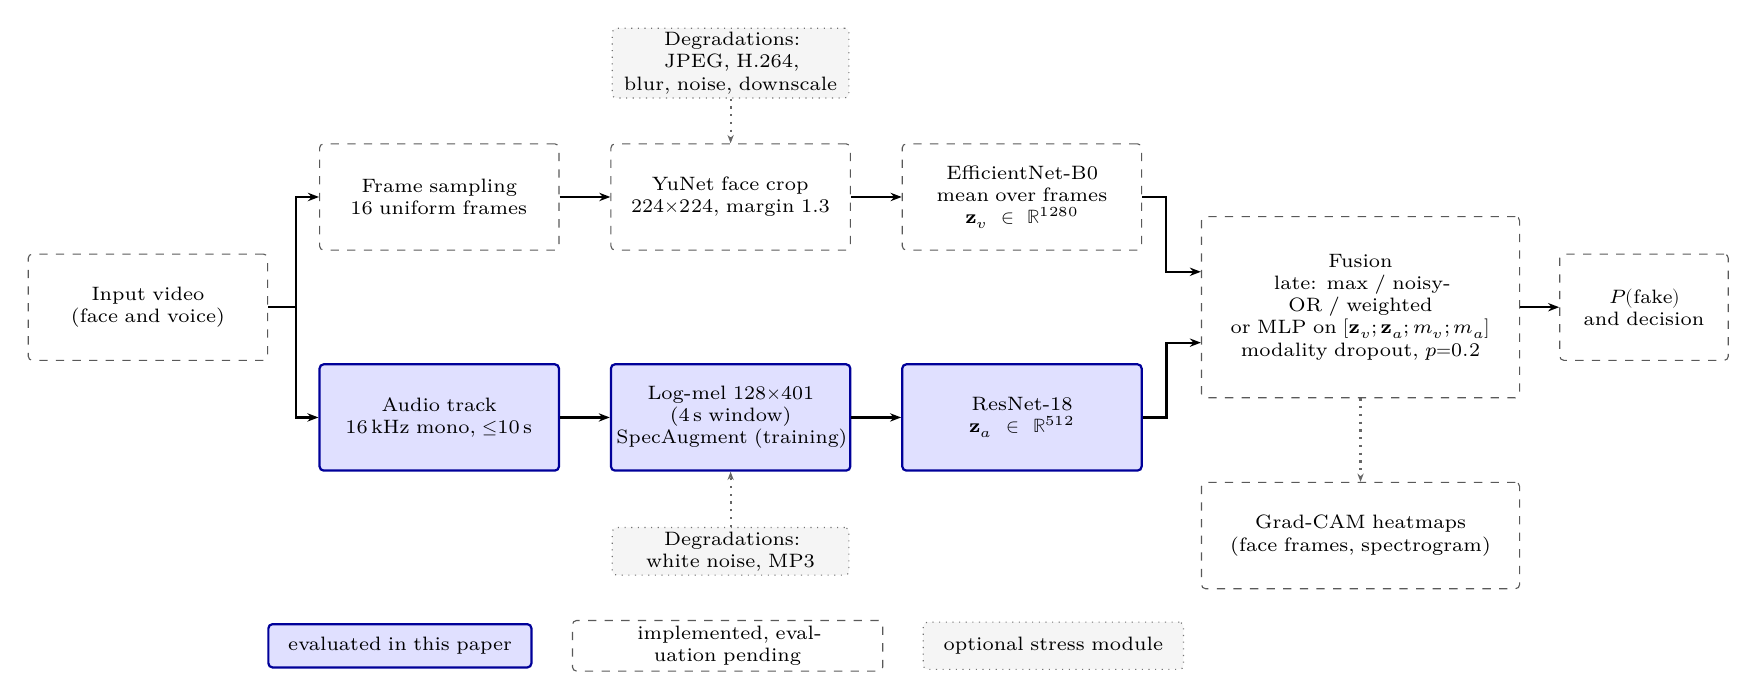
\begin{tikzpicture}[
  font=\scriptsize,
  box/.style={draw, rounded corners=1.5pt, minimum height=1.35cm, text width=2.9cm, align=center, inner sep=2pt},
  done/.style={box, fill=blue!12, draw=blue!60!black, thick},
  todo/.style={box, dashed, draw=black!65},
  deg/.style={draw, dotted, rounded corners=1.5pt, text width=2.9cm, align=center, inner sep=1.5pt, minimum height=0.6cm, draw=black!55, fill=black!4},
  arr/.style={-{Stealth[length=4pt]}, thick},
  darr/.style={-{Stealth[length=3pt]}, dotted, thick, black!60}
]
\node[todo] (in)  at (0,0)      {Input video\\(face and voice)};
\node[todo] (fr)  at (3.7,1.4)  {Frame sampling\\16 uniform frames};
\node[todo] (fc)  at (7.4,1.4)  {YuNet face crop\\$224{\times}224$, margin 1.3};
\node[todo] (vb)  at (11.1,1.4) {EfficientNet-B0\\mean over frames\\$\mathbf z_v\in\mathbb R^{1280}$};
\node[done] (au)  at (3.7,-1.4) {Audio track\\16\,kHz mono, $\leq$10\,s};
\node[done] (mel) at (7.4,-1.4) {Log-mel $128{\times}401$\\(4\,s window)\\SpecAugment (training)};
\node[done] (ab)  at (11.1,-1.4) {ResNet-18\\$\mathbf z_a\in\mathbb R^{512}$};
\node[todo, text width=3.9cm, minimum height=2.3cm] (fu) at (15.4,0) {Fusion\\late: max / noisy-OR / weighted\\or MLP on $[\mathbf z_v;\mathbf z_a;m_v;m_a]$\\modality dropout, $p{=}0.2$};
\node[todo, text width=2.0cm] (out) at (19.0,0) {$P(\mathrm{fake})$\\and decision};
\node[deg] (dv) at (7.4,3.1)  {Degradations: JPEG, H.264,\\blur, noise, downscale};
\node[deg] (da) at (7.4,-3.1) {Degradations:\\white noise, MP3};
\node[todo, text width=3.9cm] (gc) at (15.4,-2.9) {Grad-CAM heatmaps\\(face frames, spectrogram)};

\draw[arr] (in.east) -- ++(0.35,0) |- (fr.west);
\draw[arr] (in.east) -- ++(0.35,0) |- (au.west);
\draw[arr] (fr) -- (fc);
\draw[arr] (fc) -- (vb);
\draw[arr] (au) -- (mel);
\draw[arr] (mel) -- (ab);
\draw[arr] (vb.east) -- ++(0.3,0) |- ($(fu.west)+(0,0.45)$);
\draw[arr] (ab.east) -- ++(0.3,0) |- ($(fu.west)+(0,-0.45)$);
\draw[arr] (fu) -- (out);
\draw[darr] (dv) -- (fc);
\draw[darr] (da) -- (mel);
\draw[darr] (fu) -- (gc);

% legend
\node[done, text width=3.2cm, minimum height=0.55cm] (l1) at (3.2,-4.3) {evaluated in this paper};
\node[todo, text width=3.8cm, minimum height=0.55cm, right=0.5cm of l1] (l2) {implemented, evaluation pending};
\node[deg, text width=3.2cm, right=0.5cm of l2] (l3) {optional stress module};
\end{tikzpicture}}
\caption{Pipeline of the proposed detector. The two branches run in parallel and meet in a fusion stage. Shaded boxes are the components evaluated in Section~V.}
\label{fig:arch}
\end{figure*}

\subsection{Preprocessing}
\emph{Frames and faces.} Sixteen frames are sampled uniformly from each video. YuNet \cite{wu2023yunet} locates the face, the box is enlarged by a factor of 1.3, and the crop is resized to $224\times224$. A frame without a detection reuses the previous box.

\emph{Audio.} The track is decoded with ffmpeg to 16\,kHz mono and truncated to ten seconds. A 128-band mel spectrogram is computed with librosa \cite{mcfee2015librosa} using a 400-sample (25\,ms) window, a 160-sample (10\,ms) hop and a 512-point FFT, then converted to decibels with a floor of $-100$\,dB. A four-second window gives a $128\times401$ input: a random crop during training and a centre crop at test time. Each window is standardised to zero mean and unit variance,
\begin{equation}
\tilde{S}=\frac{S-\mu(S)}{\sigma(S)+\epsilon},\qquad \epsilon=10^{-5}.
\end{equation}

\subsection{Visual branch}
An ImageNet-pretrained \cite{deng2009imagenet} EfficientNet-B0 \cite{tan2019efficientnet} from the timm library \cite{wightman2019timm} encodes every valid frame $x_t$ into $\mathbf f_t\in\mathbb R^{1280}$ (4.0\,M parameters). With $\mathcal T$ the set of frames that contain a face,
\begin{equation}
\mathbf z_v=\frac{1}{|\mathcal T|}\sum_{t\in\mathcal T}\mathbf f_t,\qquad
\ell_v=\frac{1}{|\mathcal T|}\sum_{t\in\mathcal T}\mathbf w^{\top}\mathbf f_t+b .
\end{equation}
Frames without a face are masked out rather than fed to the network as blanks. The training target is the video label alone, so a real face with a cloned voice counts as real for this branch.

\subsection{Audio branch}
An ImageNet-pretrained ResNet-18 \cite{he2016resnet} treats $\tilde S$ as an image; the single channel is repeated three times so the pretrained stem can be reused. The 512-dimensional pooled embedding $\mathbf z_a$ passes through dropout (0.3) and a linear layer to give the logit $\ell_a$. The backbone has 11.2\,M parameters. SpecAugment \cite{park2019specaugment} is applied in training with two frequency masks of at most 16 bands and two time masks of at most 40 frames, filled with the window mean.

\subsection{Fusion}
Let $y_v,y_a\in\{0,1\}$ denote the face and voice labels and let the overall label be
\begin{equation}
y=y_v\lor y_a ,
\label{eq:or}
\end{equation}
that is, a clip is fake if either channel is fake. With branch probabilities $p_v=\sigma(\ell_v)$ and $p_a=\sigma(\ell_a)$, three training-free late rules are available:
\begin{align}
p_{\max}&=\max(p_v,p_a),\\
p_{\mathrm{or}}&=1-(1-p_v)(1-p_a),\\
p_{w}&=w\,p_v+(1-w)\,p_a .
\end{align}
Max and noisy-OR mirror the logical OR in \eqref{eq:or}, whereas the weighted mean dilutes a confident detection in one channel with an unsure score from the other. The rule, and $w$ in steps of 0.05, are chosen by validation AUC. The learned alternative concatenates both embeddings with two presence flags $m_v,m_a\in\{0,1\}$,
\begin{equation}
\ell=\mathbf W_2\,\mathrm{ReLU}\!\big(\mathbf W_1[\mathbf z_v;\mathbf z_a;m_v;m_a]+\mathbf b_1\big)+b_2 ,
\end{equation}
with 256 hidden units. During training one modality is hidden with probability 0.2 \cite{neverova2016moddrop}, so that clips lacking a face or a soundtrack are still handled.

\subsection{Training objective}
Each branch is trained with class-weighted binary cross-entropy,
\begin{equation}
\mathcal L=-\frac1N\sum_{i=1}^{N}\Big[\lambda\,y_i\log\sigma(\ell_i)+(1-y_i)\log\big(1-\sigma(\ell_i)\big)\Big],
\end{equation}
where $\lambda=n_{\text{real}}/n_{\text{fake}}$, which equals 1 for the balanced subset used here.

\subsection{Stress protocol}
Table~\ref{tab:degrade} lists the planned degradations. Video operations act on the face-crop sequence, which approximates platform re-encoding of the face region but is not identical to compressing whole frames before detection. Audio operations act on the stored waveform before the spectrogram is computed. Two further conditions, face-only and voice-only, remove one modality entirely. Optional robust training applies a random degradation to each sample with probability 0.5. The design follows the logic of corruption benchmarks \cite{hendrycks2019corruptions}.

\begin{table}[!t]
\caption{Planned Degradation Protocol (Implemented, Not Yet Run)}
\label{tab:degrade}
\centering
\small
\begin{tabular}{@{}llccc@{}}
\toprule
Modality & Degradation & Mild & Medium & Severe\\
\midrule
Video & JPEG quality & 90 & 50 & 20\\
Video & H.264 CRF & 23 & 30 & 40\\
Video & Gaussian blur $\sigma$ & 1 & 2 & 3\\
Video & Gaussian noise $\sigma$ & 5 & 15 & 30\\
Video & Downscale factor & $2\times$ & $3\times$ & $4\times$\\
Audio & White-noise SNR (dB) & 20 & 10 & 5\\
Audio & MP3 bitrate (kbit/s) & 64 & 32 & 16\\
\bottomrule
\end{tabular}
\end{table}

\subsection{Explanation}
For a convolutional layer with activation maps $A^{k}$, Grad-CAM \cite{selvaraju2017gradcam} weights each map by the spatially averaged gradient of the output logit $\ell$,
\begin{equation}
\alpha_k=\frac1Z\sum_{i,j}\frac{\partial \ell}{\partial A^{k}_{ij}},\qquad
L=\mathrm{ReLU}\Big(\sum_k\alpha_kA^{k}\Big),
\end{equation}
and upsamples $L$ to the input. We hook the last convolutional block of each branch (EfficientNet \texttt{bn2}, ResNet \texttt{layer4}), giving a $7\times7$ map per face and a $4\times13$ map per spectrogram. For the fused model, one backward pass of the fused logit yields maps for every face frame and for the spectrogram together.

%--------------------------------------------------------------------
\section{Experimental Setup}
\subsection{Data}
Table~\ref{tab:data} places the four datasets in the study. Only ASVspoof~2019 LA has been trained and evaluated so far. We keep its official protocol: the training, development and evaluation partitions become our train, validation and test splits (Fig.~\ref{fig:split}). Because the full partitions are large, we draw up to 2{,}500 bona fide and 2{,}500 spoofed clips per partition with seed 42, giving 5{,}000 clips per split. The training and development partitions contain attacks A01--A06. The evaluation partition contains A07--A19, of which A16 and A19 reuse the algorithms of A04 and A06 and the other eleven are unseen \cite{wang2020asvspoof}. Our test set contains 171--209 clips per attack.

\begin{table}[!t]
\caption{Datasets and Their Role in the Study}
\label{tab:data}
\centering
\footnotesize
\begin{tabular}{@{}>{\raggedright\arraybackslash}p{1.55cm}>{\raggedright\arraybackslash}p{3.35cm}>{\raggedright\arraybackslash}p{1.65cm}@{}}
\toprule
Dataset & Role & Status\\
\midrule
ASVspoof 2019 LA & Voice-branch training, per-attack testing & Used here\\
FakeAVCeleb & Main audio-visual training and test; four label categories & Access pending\\
DFDC (sample) & Pipeline development, visual baseline & Planned\\
Celeb-DF v2 & Cross-dataset test of the visual branch & Planned\\
\bottomrule
\end{tabular}
\end{table}

\begin{figure}[!t]
\centering
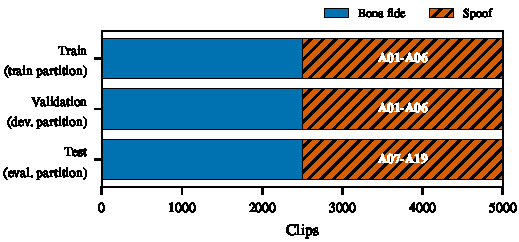
\includegraphics[width=\columnwidth]{fig_split}
\caption{ASVspoof 2019 LA subset used for the voice branch. Each split is balanced; labels inside the bars name the attack systems present.}
\label{fig:split}
\end{figure}

\subsection{Training configuration}
Table~\ref{tab:train} lists the voice-branch settings, taken from the saved run configuration. The model was trained in PyTorch \cite{paszke2019pytorch} on a single Tesla T4 GPU in Google Colab with mixed precision \cite{micikevicius2018mixed}. We used AdamW \cite{loshchilov2019adamw} with a cosine learning-rate schedule \cite{loshchilov2017sgdr}. The classifier head learns ten times faster than the backbone, and the backbone is frozen during the first epoch.

\begin{table}[!t]
\caption{Voice-Branch Training Configuration}
\label{tab:train}
\centering
\footnotesize
\begin{tabular}{@{}ll@{}}
\toprule
Item & Value\\
\midrule
Backbone & ResNet-18, ImageNet initialisation\\
Input & $128{\times}401$ log-mel, per-window standardised\\
Optimiser & AdamW, weight decay $10^{-4}$\\
Learning rate & $10^{-4}$ backbone, $10^{-3}$ head\\
Schedule & Cosine annealing, $T_{\max}=15$ epochs\\
Batch size, dropout & 32, 0.3\\
Gradient clipping & Global norm 1.0\\
Frozen backbone & First epoch\\
Early stopping & Validation AUC, patience 3\\
Augmentation & Random 4\,s crop, SpecAugment\\
Seed & 42\\
Hardware & Colab Tesla T4, PyTorch 2.11 (CUDA 13.0)\\
Time per epoch & about \SecPerEpoch\,s\\
\bottomrule
\end{tabular}
\end{table}

\subsection{Metrics and statistics}
Spoof is the positive class and each model outputs $P(\text{spoof})$. We report the area under the ROC curve (AUC) \cite{fawcett2006roc} and the equal error rate, the common value of false-alarm rate and miss rate at the threshold where they meet. A detection error trade-off (DET) view \cite{martin1997det} is also provided. At fixed thresholds we give accuracy, precision, recall and F1. Calibration is summarised by the expected calibration error over $M=15$ equal-width bins \cite{naeini2015ece},
\begin{equation}
\mathrm{ECE}=\sum_{m=1}^{M}\frac{|B_m|}{n}\,\big|\mathrm{acc}(B_m)-\mathrm{conf}(B_m)\big|,
\end{equation}
together with the Brier score \cite{brier1950} and the negative log-likelihood. Confidence intervals are percentile intervals from 2{,}000 stratified bootstrap resamples of the test clips \cite{efron1993bootstrap}. These intervals describe sampling variation of the test set only; they do not capture training randomness, since a single seed was run. Per-attack figures score each attack's clips against all 2{,}500 bona fide test clips.

\subsection{Planned experiments}
Table~\ref{tab:plan} lists the full evaluation programme and what has been done. Experiment E1 is the one reported in Section~V. The others reuse the same code, metrics and statistical procedure, so their results will be directly comparable once the data are available.

\begin{table}[!t]
\caption{Evaluation Programme and Status}
\label{tab:plan}
\centering
\footnotesize
\begin{tabular}{@{}>{\raggedright\arraybackslash}p{0.55cm}>{\raggedright\arraybackslash}p{3.3cm}>{\raggedright\arraybackslash}p{1.7cm}@{}}
\toprule
ID & Experiment & Status\\
\midrule
E1 & Voice branch on ASVspoof 2019 LA, per-attack and calibration analysis & Done (Sec.~V)\\
E2 & Face branch on DFDC and FakeAVCeleb; transfer to Celeb-DF & Pending data\\
E3 & Voice branch fine-tuned on FakeAVCeleb with and without ASVspoof pre-training & Pending data\\
E4 & Visual-only, audio-only, late and intermediate fusion on the same test clips, overall and per category & Pending E2, E3\\
E5 & Degradation sweep (Table~\ref{tab:degrade}), missing-modality tests, standard versus robust training & Pending E4\\
E6 & Grad-CAM gallery and faithfulness checks & Pending E4\\
\bottomrule
\end{tabular}
\end{table}

\subsection{Model selection and test use}
The checkpoint with the best validation AUC was evaluated on the test split once. No hyper-parameter was tuned on test data. The EER threshold is, by definition, computed from the test scores, so metrics at that threshold are post-hoc diagnostics and not attainable operating points.

%--------------------------------------------------------------------
\section{Results and Analysis}
\subsection{Training behaviour}
Fig.~\ref{fig:train} shows the run. Training loss fell steadily. Validation AUC jumped from 0.855 to 0.99999 once the backbone was unfrozen, and reached exactly 1.0 at epoch 3. Because later epochs never improved on that value, the patience counter expired after epoch 6 and the epoch-3 checkpoint was kept. The six epochs took \TrainMinutes{} minutes in total.

Table~\ref{tab:history} lists the per-epoch values behind the figure.

\begin{table}[!t]
\caption{Epoch-by-Epoch Training Log of the Voice Branch}
\label{tab:history}
\centering
\footnotesize
\resizebox{\columnwidth}{!}{\begin{tabular}{@{}cccccrr@{}}
\toprule
Epoch & Train loss & Val. loss & Val. AUC & Val. acc. (\%) & LR & Time (s)\\
\midrule
1 & 0.6428 & 0.5526 & 0.854869 & 70.30 & 9.90e-05 & 158 \\
2 & 0.1940 & 0.0032 & 0.999998 & 99.94 & 9.60e-05 & 160 \\
3 & 0.0367 & 0.0047 & 1.000000 & 99.84 & 9.00e-05 & 158 \\
4 & 0.0102 & 0.0026 & 1.000000 & 99.90 & 8.30e-05 & 157 \\
5 & 0.0173 & 0.0005 & 1.000000 & 99.98 & 7.50e-05 & 156 \\
6 & 0.0095 & 0.0003 & 1.000000 & 100.00 & 6.50e-05 & 154 \\
\bottomrule
\end{tabular}
}
\par\smallskip{\scriptsize LR is the value logged at the end of each epoch (cosine schedule, backbone group).}
\end{table}

The validation curve is the first warning sign. The development partition shares its six attack systems with the training partition, so near-perfect validation scores only show that the model has learned those six. The test AUC of \AUC{}, drawn as a horizontal line in Fig.~\ref{fig:train}, sits below every validation point from epoch 2 onward.

\begin{figure}[!t]
\centering
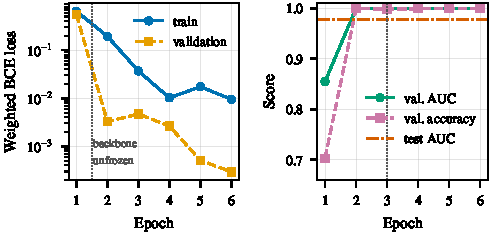
\includegraphics[width=\columnwidth]{fig_training}
\caption{Left: training and validation loss per epoch (log scale). Right: validation AUC and accuracy against the final test AUC. The dotted line at epoch 3 marks the selected checkpoint.}
\label{fig:train}
\end{figure}

\subsection{Aggregate test performance}
Table~\ref{tab:main} gives the headline numbers and Fig.~\ref{fig:roc} the corresponding curves. The model ranks spoofed speech above bona fide speech with an AUC of \AUC{} (\AUClo--\AUChi). The EER is \EER\% (\EERlo--\EERhi\%).

The pooled figures hide a split. Excluding A17, the AUC rises to \AUCexcl{} and the EER falls to \EERexcl\%. A17 alone has an AUC of \AUCAsev{} and an EER of \EERAsev\% (bootstrap interval \EERAsevlo--\EERAsevhi\%). In the DET plot of Fig.~\ref{fig:roc} the A17 curve crosses the equal-error diagonal near 34\%, far from the other two curves.

\begin{table}[!t]
\caption{Test Results on the ASVspoof 2019 LA Evaluation Subset ($n=5{,}000$)}
\label{tab:main}
\centering
\footnotesize
\begin{tabular}{@{}lc@{}}
\toprule
Metric & Value (95\% CI)\\
\midrule
AUC & \AUC{} (\AUClo--\AUChi)\\
EER (\%) & \EER{} (\EERlo--\EERhi)\\
Accuracy at threshold 0.5 (\%) & 91.24\\
Precision / recall at 0.5 & 0.991 / 0.832\\
F1 at 0.5 & 0.905\\
Accuracy at EER threshold (\%)$^{*}$ & \AccEER\\
\midrule
AUC excluding A17 & \AUCexcl\\
EER excluding A17 (\%) & \EERexcl\\
EER on A17 only (\%) & \EERAsev{} (\EERAsevlo--\EERAsevhi)\\
\midrule
Brier score / NLL & \Brier{} / \NLL\\
ECE (15 bins) & \ECE\\
\bottomrule
\multicolumn{2}{@{}p{0.97\columnwidth}@{}}{\scriptsize $^{*}$Threshold \EERthr{} was chosen on the test scores, so this is a diagnostic and not a deployable setting.}
\end{tabular}
\end{table}

\begin{figure}[!t]
\centering
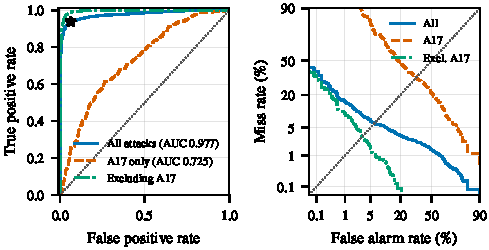
\includegraphics[width=\columnwidth]{fig_roc_det}
\caption{ROC (left) and DET (right) curves for all attacks, for A17 alone and for all attacks except A17. The star marks the EER operating point. DET axes are probit-scaled.}
\label{fig:roc}
\end{figure}

\subsection{Operating point}
At the default threshold of 0.5 the detector accepts \,99.2\% of bona fide clips (19 false alarms in 2{,}500) but catches only 83.2\% of spoofs; 419 spoofed clips are missed (Fig.~\ref{fig:conf}). The error is lopsided: a false-alarm rate of \FPRhalf\% against a miss rate of \FNRhalf\%. Fig.~\ref{fig:scores} shows why. Bona fide scores pile up near zero, but a long tail of spoofs sits at low and intermediate scores. At the EER threshold the two error rates match at 6.2\%, yet that threshold is as low as \EERthr{}, and it flags 155 bona fide clips where the default flags 19. Fig.~\ref{fig:calib} (right) plots both error rates against the threshold; the default 0.5 lies in a region where the miss rate rises steeply.

\begin{figure}[!t]
\centering
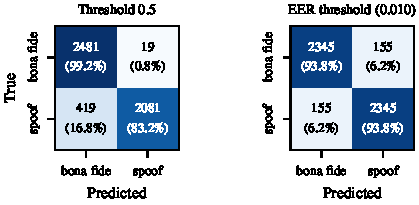
\includegraphics[width=\columnwidth]{fig_confusion}
\caption{Confusion matrices at the default threshold (left) and at the post-hoc EER threshold (right). Cell values give counts and the share of the true class.}
\label{fig:conf}
\end{figure}

\begin{figure}[!t]
\centering
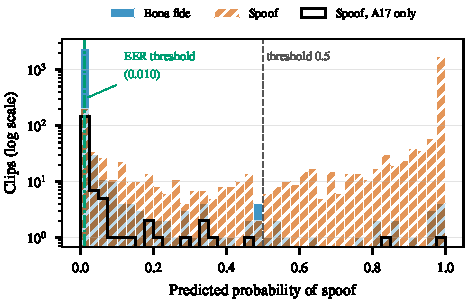
\includegraphics[width=\columnwidth]{fig_scores}
\caption{Distribution of predicted spoof probability on the test set (log-scaled counts). The black outline shows A17 spoofs only. The dashed line marks the default threshold and the dash-dot line marks the EER threshold.}
\label{fig:scores}
\end{figure}

\subsection{Behaviour per attack system}
Table~\ref{tab:attack} and Fig.~\ref{fig:attack} break the result down. Eight of thirteen attacks are caught in at least 94\% of clips. These include A16 and A19, whose generation algorithms appeared in training; pooled, their EER is \EERseen\%. The unseen attacks other than A17 trail them, with a pooled EER of \EERunseen\% (AUC \AUCunseen). Familiarity with the algorithm therefore helps, but it is not the whole story: A07--A09 are unseen and are still detected almost perfectly.

Three groups stand out. A07--A09, A11 and A14 are detected almost perfectly even though they are unseen. A10, A12, A13 and A18 are detected in 64--80\% of clips at threshold 0.5 while keeping EERs near 4--5\%, which means their scores rank correctly but fall on the wrong side of the default threshold. A17 is different in kind: \DetAsev\% of its clips cross 0.5 and its AUC of \AUCAsev{} shows poor ranking as well. It accounts for 169 of the 419 missed spoofs (40\%) while making up 7\% of the spoofed test clips.

\begin{table}[!t]
\caption{Per-Attack Results (Each Attack Against All 2{,}500 Bona Fide Test Clips)}
\label{tab:attack}
\centering
\footnotesize
\begin{tabular}{@{}lrrrcr@{}}
\toprule
Attack & $n$ & Detected (\%) & Median score & AUC & EER (\%)\\
\midrule
A07 & 194 & 100.0 & 1 & 1.0000 & 0.06 \\
A08 & 182 & 100.0 & 1 & 1.0000 & 0.08 \\
A09 & 189 & 100.0 & 1 & 1.0000 & 0.10 \\
A10 & 209 & 69.4 & 0.856 & 0.9851 & 5.19 \\
A11 & 197 & 100.0 & 1 & 0.9997 & 0.79 \\
A12 & 205 & 79.5 & 0.963 & 0.9915 & 4.30 \\
A13 & 204 & 64.2 & 0.692 & 0.9888 & 4.41 \\
A14 & 182 & 100.0 & 1 & 0.9999 & 0.45 \\
A15 & 189 & 94.2 & 1 & 0.9979 & 2.14 \\
A16$^\dagger$ & 178 & 100.0 & 1 & 0.9999 & 0.08 \\
A17 & 171 & 1.2 & 0.000548 & 0.7248 & 34.37 \\
A18 & 207 & 71.5 & 0.9 & 0.9884 & 4.90 \\
A19$^\dagger$ & 193 & 99.5 & 1 & 0.9988 & 0.40 \\
\bottomrule
\multicolumn{6}{@{}p{0.97\columnwidth}@{}}{\scriptsize $^\dagger$Same generation algorithm as a training attack (A04 / A06). ``Detected'' uses threshold 0.5.}
\end{tabular}

\end{table}

\begin{figure}[!t]
\centering
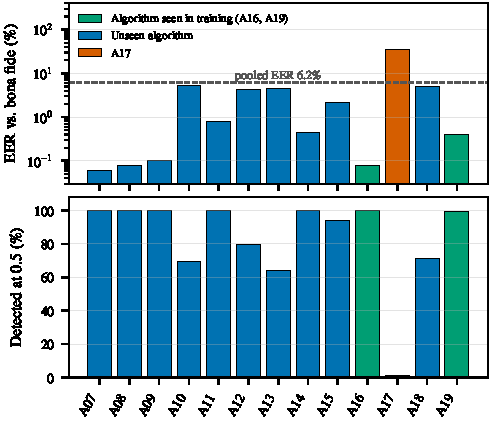
\includegraphics[width=\columnwidth]{fig_per_attack}
\caption{EER (log scale, top) and detection rate at threshold 0.5 (bottom) for each attack system. The dashed line is the pooled EER.}
\label{fig:attack}
\end{figure}

Fig.~\ref{fig:ecdf} compares score distributions directly. The A17 curve sits to the right of the bona fide curve, which is why its AUC is above 0.5, but both stay low: 77\% of A17 clips score below the EER threshold, against 94\% of bona fide clips, and about 82\% of A17 clips score below the 95th percentile of bona fide scores. The model treats most A17 clips as ordinary speech and does not flag them as uncertain. The remaining attacks are separated from bona fide speech by several orders of magnitude.

\begin{figure}[!t]
\centering
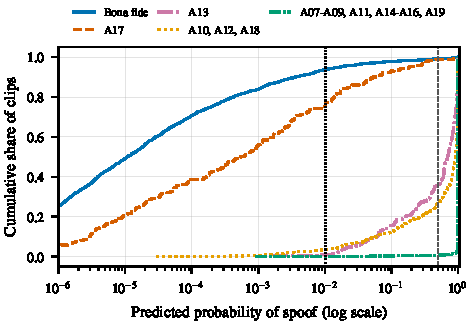
\includegraphics[width=\columnwidth]{fig_score_ecdf}
\caption{Empirical cumulative distribution of predicted spoof probability for bona fide speech and for groups of attacks (log-scaled $x$ axis). Dashed and dotted vertical lines mark thresholds 0.5 and \EERthr{}.}
\label{fig:ecdf}
\end{figure}

\subsection{Calibration}
The reliability curve in Fig.~\ref{fig:calib} (left) departs clearly from the diagonal, with an ECE of \ECE{}. The largest deviation comes from the lowest-probability bin, which supplies about 0.049 of the 0.083 total. It holds 2{,}683 clips, of which 253 (9.4\%) are spoofs, although the mean predicted probability in the bin is 0.002. In other words, a score near zero is not a reliable promise of authenticity on unseen attacks. This is consistent with the general finding that modern networks are poorly calibrated \cite{guo2017calibration}, with the specific pattern here being an under-estimate of spoof risk at the low end of the score range.

\begin{figure}[!t]
\centering
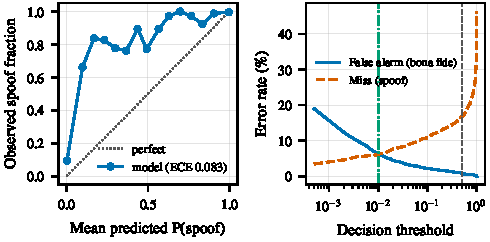
\includegraphics[width=\columnwidth]{fig_calibration_threshold}
\caption{Left: reliability curve with 15 bins. Right: false-alarm and miss rates as a function of the decision threshold (log scale). Vertical lines mark threshold 0.5 (dashed) and the EER threshold (dash-dot).}
\label{fig:calib}
\end{figure}

\subsection{Qualitative explanation}
Fig.~\ref{fig:cam} shows a Grad-CAM overlay for a clip synthesised with a built-in operating-system text-to-speech voice. The clip was run through the public demo and is not part of the evaluation set; the model scored it as spoofed with probability near 1. The strongest response covers a mid-band region in the first half of the window. We offer this only as an illustration of the interface. No faithfulness test, such as parameter randomisation \cite{adebayo2018sanity}, has been run on the trained model, and a $4\times13$ map cannot localise individual artefacts.

\begin{figure}[!t]
\centering
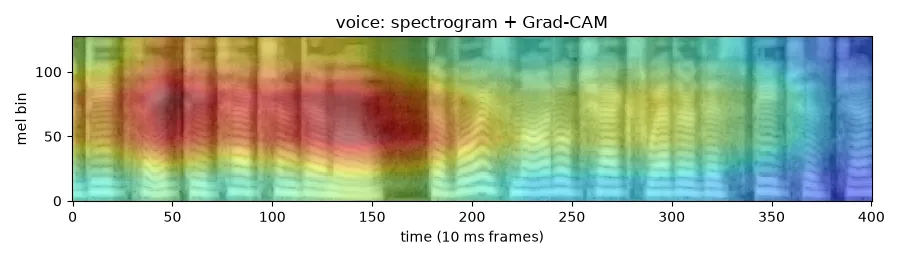
\includegraphics[width=\columnwidth]{fig_gradcam_voice}
\caption{Grad-CAM overlay on the log-mel spectrogram for an informal demonstration clip (system text-to-speech, outside the test set). Warm colours indicate regions that raised the spoof score.}
\label{fig:cam}
\end{figure}

%--------------------------------------------------------------------
\section{Discussion}
Table~\ref{tab:summary} condenses the findings and the caveat attached to each; the paragraphs below expand on them.

\begin{table*}[!t]
\caption{Summary of Findings and Their Caveats}
\label{tab:summary}
\centering
\footnotesize
\begin{tabular}{@{}>{\raggedright\arraybackslash}p{4.4cm}>{\raggedright\arraybackslash}p{6.4cm}>{\raggedright\arraybackslash}p{5.6cm}@{}}
\toprule
Finding & Evidence & Caveat\\
\midrule
Overall separation is strong & AUC \AUC{} (\AUClo--\AUChi), EER \EER\% (Table~\ref{tab:main}) & Subset of the benchmark; one seed\\
Validation was uninformative & Val.\ AUC 1.0 from epoch 3 (Table~\ref{tab:history}) & Dev.\ partition shares attacks with training\\
One attack dominates the errors & A17: \DetAsev\% detected, EER \EERAsev\% (Table~\ref{tab:attack}) & Cause not isolated; no ablation run\\
Default threshold misses spoofs & Miss rate \FNRhalf\% against false alarms \FPRhalf\% (Fig.~\ref{fig:conf}) & EER threshold is chosen on test data\\
Low scores are not safe & 9.4\% of the lowest-score bin are spoofs (Fig.~\ref{fig:calib}) & Binned ECE depends on bin choice\\
Fusion and robustness unknown & Experiments E2--E6 not run (Table~\ref{tab:plan}) & No claim is made\\
\bottomrule
\end{tabular}
\end{table*}

\emph{Why validation failed.} The development partition reuses the training attacks, so validation AUC saturated at 1.0 and offered no basis for choosing a checkpoint or a threshold. Any checkpoint after epoch 2 looked equally good, while test behaviour on unseen attacks may differ between them. A validation split built by holding out whole attack families, for instance leave-one-attack-out, would restore a useful signal; this is the most important methodological change we would make.

\emph{A17.} The dataset paper describes A17 as a voice-conversion system that shares its VAE-based acoustic model with training attack A05 but replaces the WORLD vocoder with direct waveform filtering \cite{wang2020asvspoof}. Baseline GMM countermeasures distributed with the dataset also struggled with A17, A13 and A10 \cite{wang2020asvspoof}, so its difficulty is not unique to our model. Our results do not isolate a cause. A13, which also uses waveform filtering, is detected with an EER of 4.4\%, and A18, which also converts human speech, reaches 4.9\%, so neither the vocoder family nor the human-source input explains A17 alone. One hypothesis is that filtering a genuine utterance leaves the fine structure of natural speech largely intact, giving a vocoder-artefact detector little to find. Testing it would need ablations that we have not run.

\emph{Threshold.} The gap between the default threshold and the EER threshold, and the large shift between them (0.5 versus \EERthr), mean that reporting accuracy at 0.5 alone would hide the real sensitivity. A deployable threshold must come from data that contain unseen attacks, which again points to a better validation design.

\emph{Comparability.} Results use a 5{,}000-clip subset per partition and a single seed, so they should not be compared with published full-benchmark EERs. Our random subset also changes the per-attack mix relative to the full evaluation partition.

\emph{Out-of-domain behaviour.} In an informal check through the demo, two clips from a built-in text-to-speech voice were both flagged as spoofed. No out-of-domain bona fide recording has been tested, so the false-alarm rate on everyday microphones is unknown; this check is not evidence of generalisation.

\emph{Threats to validity.} Bootstrap intervals reflect test-sample variation, not seed variation. Each attack has fewer than 210 test clips, so per-attack EERs below 1\% rest on very few errors and should be read as ``small'' rather than as precise values. The balanced subset also removes the class imbalance found in the full protocol, which affects precision-type metrics.

\emph{What remains.} The face branch, both fusion schemes, the degradation protocol and the fused Grad-CAM analysis are implemented and tested on synthetic inputs but have not been run on real audio-visual data. Until they are, nothing in this paper supports a claim that fusion improves detection or that robust training helps.

%--------------------------------------------------------------------
\section{Conclusion}
We presented a modular audio-visual deepfake detector together with its training, stress-testing and explanation tooling, and reported the first completed experiment, a ResNet-18 voice branch on a balanced ASVspoof~2019 LA subset. The model separates bona fide from spoofed speech well overall (AUC \AUC, EER \EER\%), but one unseen attack, A17, is mostly treated as genuine speech, and a default threshold of 0.5 misses a sixth of all spoofs. Because validation shared its attacks with training, it predicted none of this. Next steps are to run the face, fusion and robustness experiments on FakeAVCeleb and Celeb-DF, to build validation sets with held-out attack families, to calibrate thresholds on such sets, and to compare the current spectrogram CNN with self-supervised and graph-attention countermeasures \cite{jung2022aasist,tak2022wav2vec}.

\section*{Reproducibility}
Code, tests, notebooks and the trained voice checkpoint are available at \url{https://github.com/tanishq1101/robust-multimodal-deepfake}. Every number in Section~V is computed from the run's saved \texttt{history.csv}, \texttt{predictions.csv} and \texttt{metrics.json} by \texttt{paper/make\_figures.py}. The interactive demo uses Gradio \cite{abid2019gradio}.

\appendices
\section{Repository Structure}
Table~\ref{tab:repo} maps each stage of the pipeline to its code module. The test suite (82 tests at the time of writing) runs on synthetic video and audio, so it needs no dataset and can be run on a laptop before any Colab session is started.

\begin{table}[!t]
\caption{Code Modules and Their Responsibilities}
\label{tab:repo}
\centering
\footnotesize
\begin{tabular}{@{}>{\raggedright\arraybackslash}p{1.9cm}>{\raggedright\arraybackslash}p{5.3cm}@{}}
\toprule
Module & Responsibility\\
\midrule
\texttt{data} & Resumable dataset downloads with checksum verification, unified manifests, identity-grouped splits\\
\texttt{preprocessing} & Frame sampling, YuNet face crops, 16\,kHz audio, log-mel spectrograms, parallel resumable batch runner\\
\texttt{datasets} & PyTorch datasets with missing-modality flags and optional SpecAugment\\
\texttt{models} & Face branch, voice branch, late and intermediate fusion\\
\texttt{training} & Shared engine: mixed precision, gradient clipping, resumable checkpoints, early stopping\\
\texttt{evaluation} & AUC, EER, threshold metrics, per-category tables, model comparison, ROC plots\\
\texttt{robustness} & Seven degradations at three severities, applied to face crops or waveforms\\
\texttt{explainability} & Hook-based Grad-CAM for single branches and for the fused model\\
\texttt{demo}, \texttt{inference} & Gradio application and command-line analysis of uploaded videos\\
\bottomrule
\end{tabular}
\end{table}

\section{Metric Conventions}
Throughout the paper, label 1 means spoof and every score is the model's probability of spoof. The false-alarm rate is the share of bona fide clips scored at or above the threshold, and the miss rate is the share of spoofed clips scored below it. The EER is the value at which these two rates are equal; when the two curves do not cross exactly on the finite test set, we average the two rates at the nearest point. AUC is the probability that a randomly chosen spoofed clip receives a higher score than a randomly chosen bona fide clip. For per-attack results, bona fide clips are always the full set of 2{,}500, so the AUC and EER of different attacks share one negative class and can be compared directly.

\bibliographystyle{IEEEtran}
\bibliography{references}

\end{document}
